Den heutigen Projektablauf bei der allink könnte man am Besten als ``natürliches Vorgehen''
umschreiben. Ein potentielles Projekt kommt an einen Partner heran, entweder über 
eine Anfrage oder eine Akquisition, der spricht sich mit den anderen Partner ab 
und nimmt dann die Mitarbeiter mit in das Projekt, die er als nötig erachtet.
Dies kommt einem Projektmanamgement organisiert über die Linie aus der Theorie
am nächsten.

Der Projektablauf wird in drei Prozesse, die Projektannahme und Offertenerstellung,
die Projektdurchführung und der Projektabschluss unterteilt und dazu werden nun die 
Ablaufdiagramme erstellt. Darin wird jede Aktion mit einer eindeutigen Nummer versehen,
um danach darauf im beschreibenden Text verweisen zu können. Nach einer Entscheidung erhöht
sich die Laufnummer jeweils um eine ganze Zahl, um die verschiedenen Wege hervorzuheben.
Zusätzlich werden die Abläufe um die Tools, die verwendet werden, ergänzt.
Es werden nicht immer alle erwähnten Tools in dem selben Projekt eingesetzt,
jedoch Projektübergreifend betrachtet, kommen alle mal beim zugeordneten Schritt 
zum Einsatz. Die verwendete Software wird zu einem späteren Zeitpunkt separat
behandelt, da es zu diesem Zeitpunkt das ``Wie?'' und nicht ``Womit?'' betrachtet
wird.

\clearpage

\subsection{Projektannahme und Offertenerstellung}

\begin{figure}[p]
\begin{center}
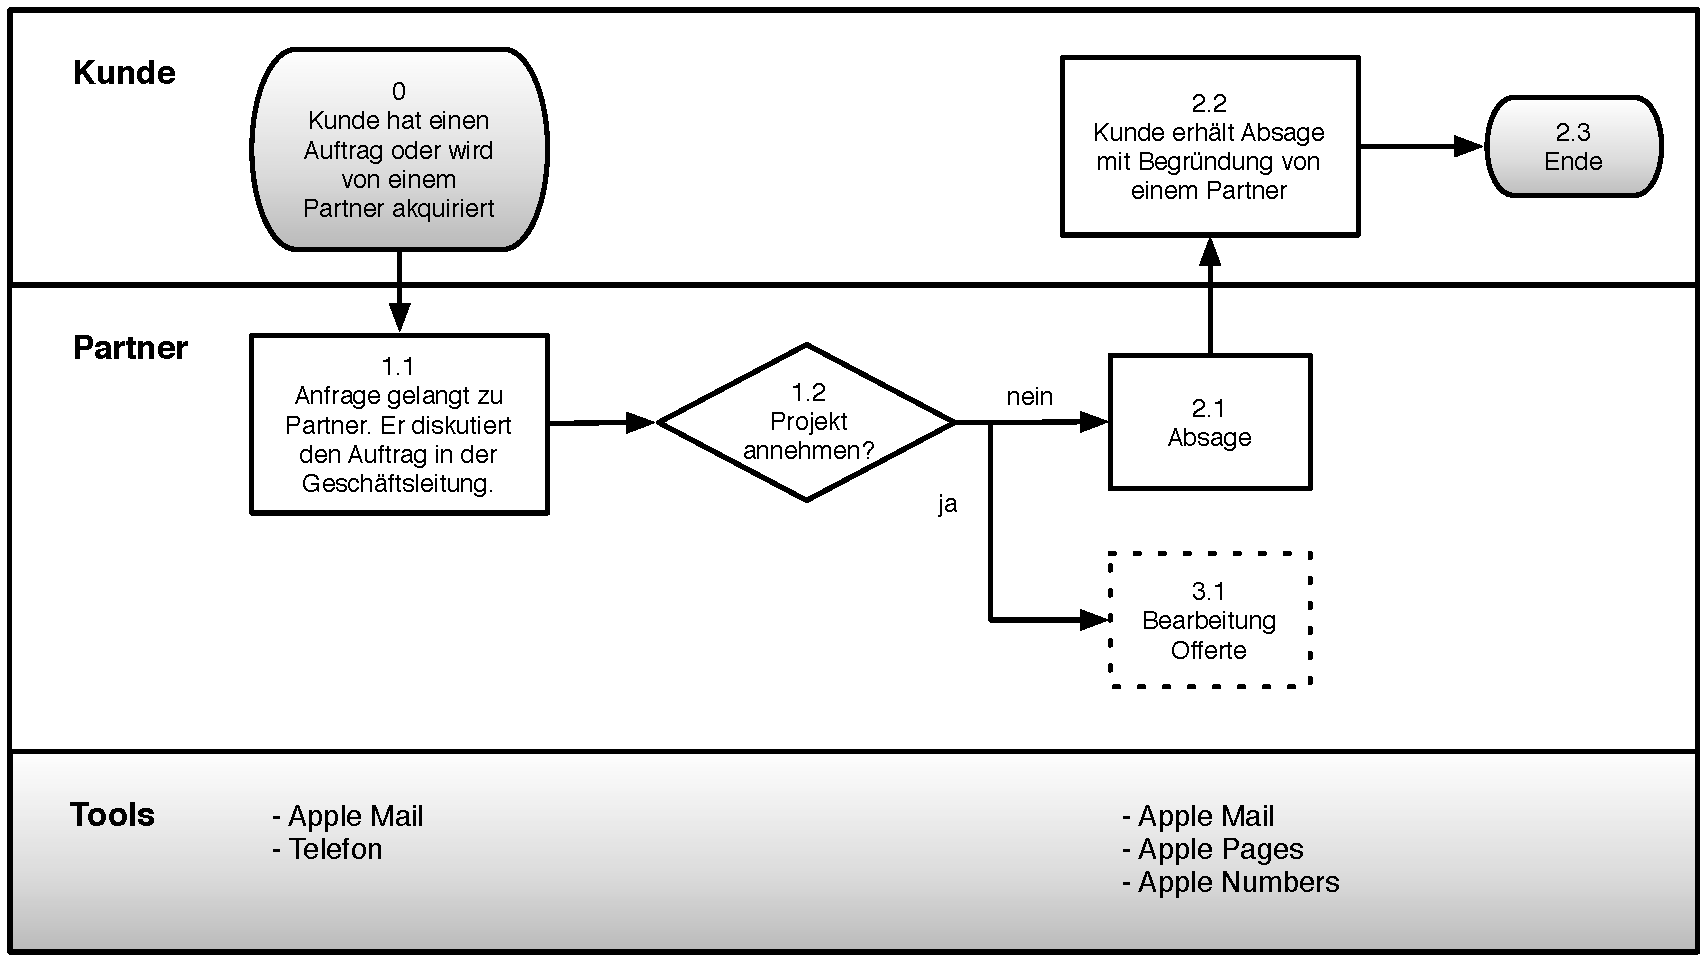
\includegraphics[width=0.99\textwidth,angle=0]{./bilder/analyse/01_ist_prozesse_offerte_01.pdf}
\caption[Offertenerstellungs Prozess von allink 1/2]{Offertenerstellungs 
    Prozess von allink 1/2\footnotemark}
\label{pic:01_ist_prozesse_offerte_01}
\end{center}
\end{figure}
\footnotetext{Eigene Darstellung}

\begin{figure}[p]
\begin{center}
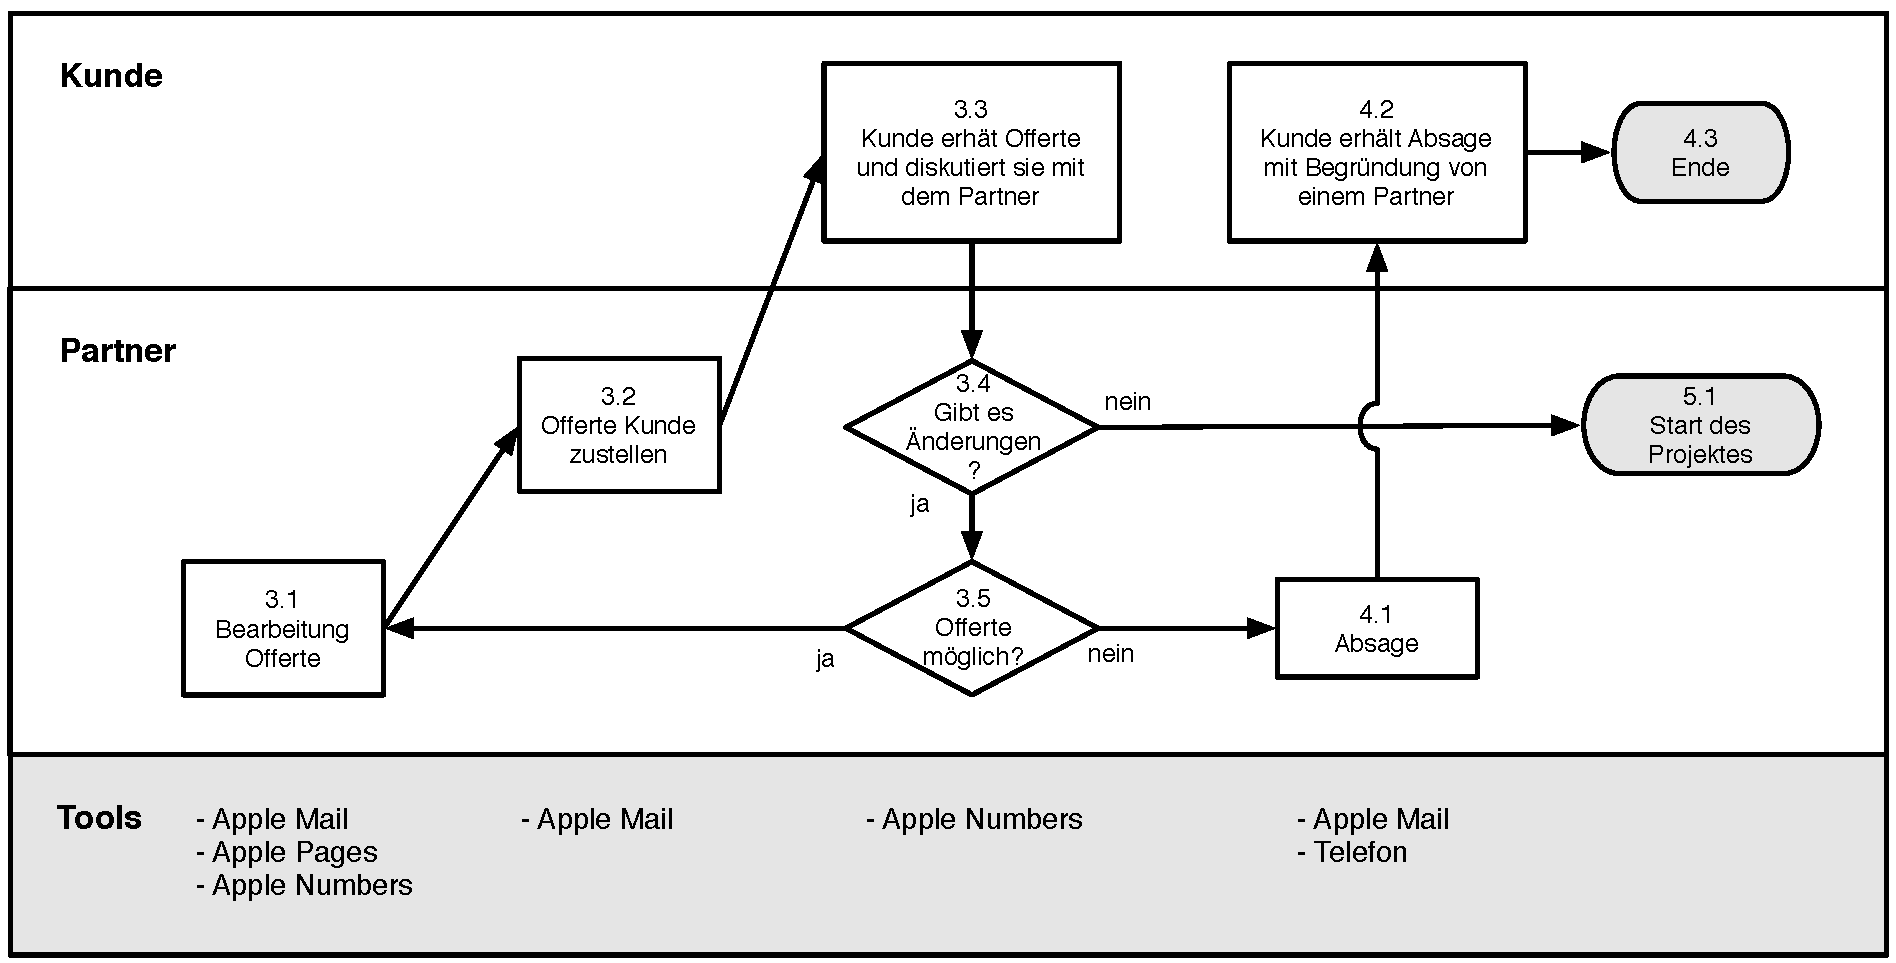
\includegraphics[width=0.99\textwidth,angle=0]{./bilder/analyse/01_ist_prozesse_offerte_02.pdf}
\caption[Offertenerstellungs Prozess von allink 2/2]{Offertenerstellungs 
    Prozess von allink 2/2\footnotemark}
\label{pic:01_ist_prozesse_offerte_02}
\end{center}
\end{figure}
\footnotetext{Eigene Darstellung}

In den Darstellungen \ref{pic:01_ist_prozesse_offerte_01} und
\ref{pic:01_ist_prozesse_offerte_02} ist der aktuelle Prozess der Offertenerstellung 
ersichtlich. Die darin verwickelten Akteuere sind der Kunde und der bzw. die Partner.
Hier werden aus der Theorie Teile der Projektdefinition und Projektplanung abgedeckt.
Eine Projektanfrage endet entweder in einer Absage oder einem Start eines neuen 
Projektes. Wenn das Projekt nicht zustande kommt, werden zurzeit die Aufwände der
Akquisition und der Offertenerstellung vernachlässigt und somit von
den durchgeführten Projekten getragen.

Als Start eines Projektablaufes wird entweder ein neues Projekt akquiriert, 
durch eine direkte Anfrage an ein Unternehmen oder einen Pitch\footnote{Als Pitch 
wird der Wettbewerb zwischen verschiedenen Agenturen um einen Auftrag eines 
Unternehmens bezeichnet.}, oder eine Anfrage kommt direkt von einem Kunden (\textbf{0}). 
Die Projekte gelangen zum heutigen Zeitpunkt immer als erstes zu einem Partner. 
Sehr selten bringt ein Mitarbeiter durch einen seiner Kontakte ein Projekt ein. 
Aber auch in diesem Fall, würde es als erstes an einen Partner herangetragen.
Dieser diskutiert den möglichen Auftrag mit den anderen Partnern in der 
Geschäftsleitung (\textbf{1.1}). Diese entscheide demokratisch ob ein Projekt 
angenommen oder abgelehnt wird (\textbf{1.2}). Sofern nicht alle Partner anwesend 
sein können, haben die anderen Partner die Kompetenz, alleine zu entscheiden.

Im Falle einer Absage (\textbf{2.1}) tritt ein Partner wieder mit dem Kunden in Kontakt.
In den meisten Fällen natürlich der Partner, der bereits mit dem Kunden Kontakt
hatte. Dem Kunden wird erklärt, aus welchen Gründen das Projekt nicht angenommen
und durchgeführt werden kann (\textbf{2.2}).

Sollte das Projekt angenommen werden, wird auf Grund den zu erbringenden
Dienstleistungen eine möglichst genaue Offerte erstellt (\textbf{3.1}). Diese Schätzungen
basieren überwiegend auf Erfahrungswerten aus anderen Projekten. Dieses Verfahren
wird in der Theorie ebenfalls empfohlen. Es wäre jedoch sinnvoll öfters auch
die Erfahrungen von Experten zum Thema heranzuziehen. 
Die Offerte wird dann dem Kunden zugestellt (\textbf{3.2}). In vielen Fällen wird dem Kunden
die Offerte präsentiert und genauer erklärt.
Der Kunde diskutiert dann mit dem oder den Partnern die Offerte (\textbf{3.3}) und bringt
bei bedarf Änderungen und Wünsche an.
Kann man sich mit dem Kunden nicht einigen, also wünscht der Kunde Änderungen
an der Offerte oder den zu erbringenden Dienstleistungen (\textbf{3.4}), die von unserer Seite
nicht mehr möglich sind (\textbf{3.5}), muss das Projekt abgesagt werden (\textbf{4.1}).
Dem Kunden wird erklärt, aus welchen Gründen die Offerte nicht angepasst oder
die Dienstleistung nicht erbracht werden kann (\textbf{4.2}).

Im Falle einer Einigung und einer Auftragserteilung startet das eigentliche
Projekt (\textbf{5.1}).

\clearpage

\subsection{Projektdurchführung}

\begin{figure}[p]
\begin{center}
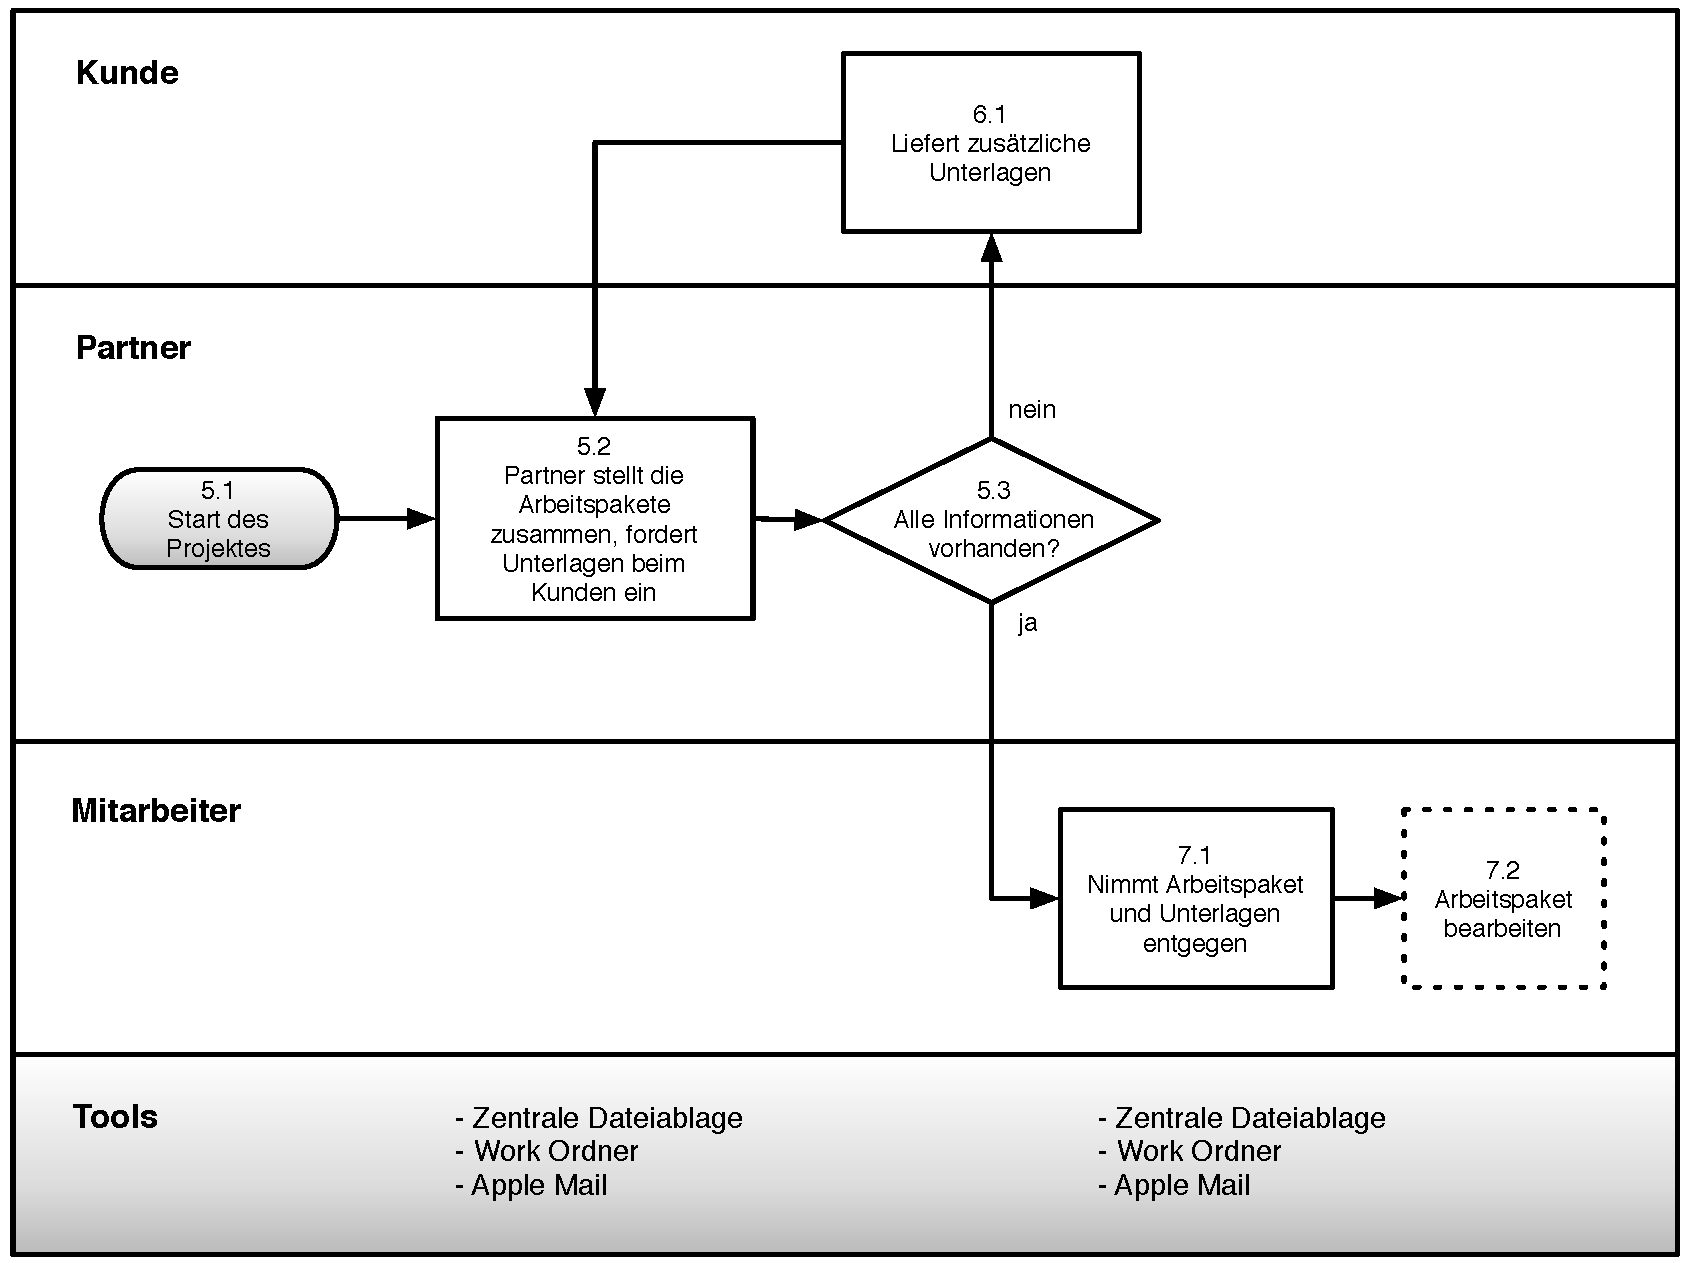
\includegraphics[width=0.99\textwidth,angle=0]{./bilder/analyse/02_ist_prozesse_arbeit_01.pdf}
\caption[Projektumsetzungs Prozess von allink 1/2]{Projektumsetzungs 
    Prozess von allink 1/2\footnotemark}
\label{pic:02_ist_prozesse_arbeit_01}
\end{center}
\end{figure}
\footnotetext{Eigene Darstellung}

\begin{figure}[p]
\begin{center}
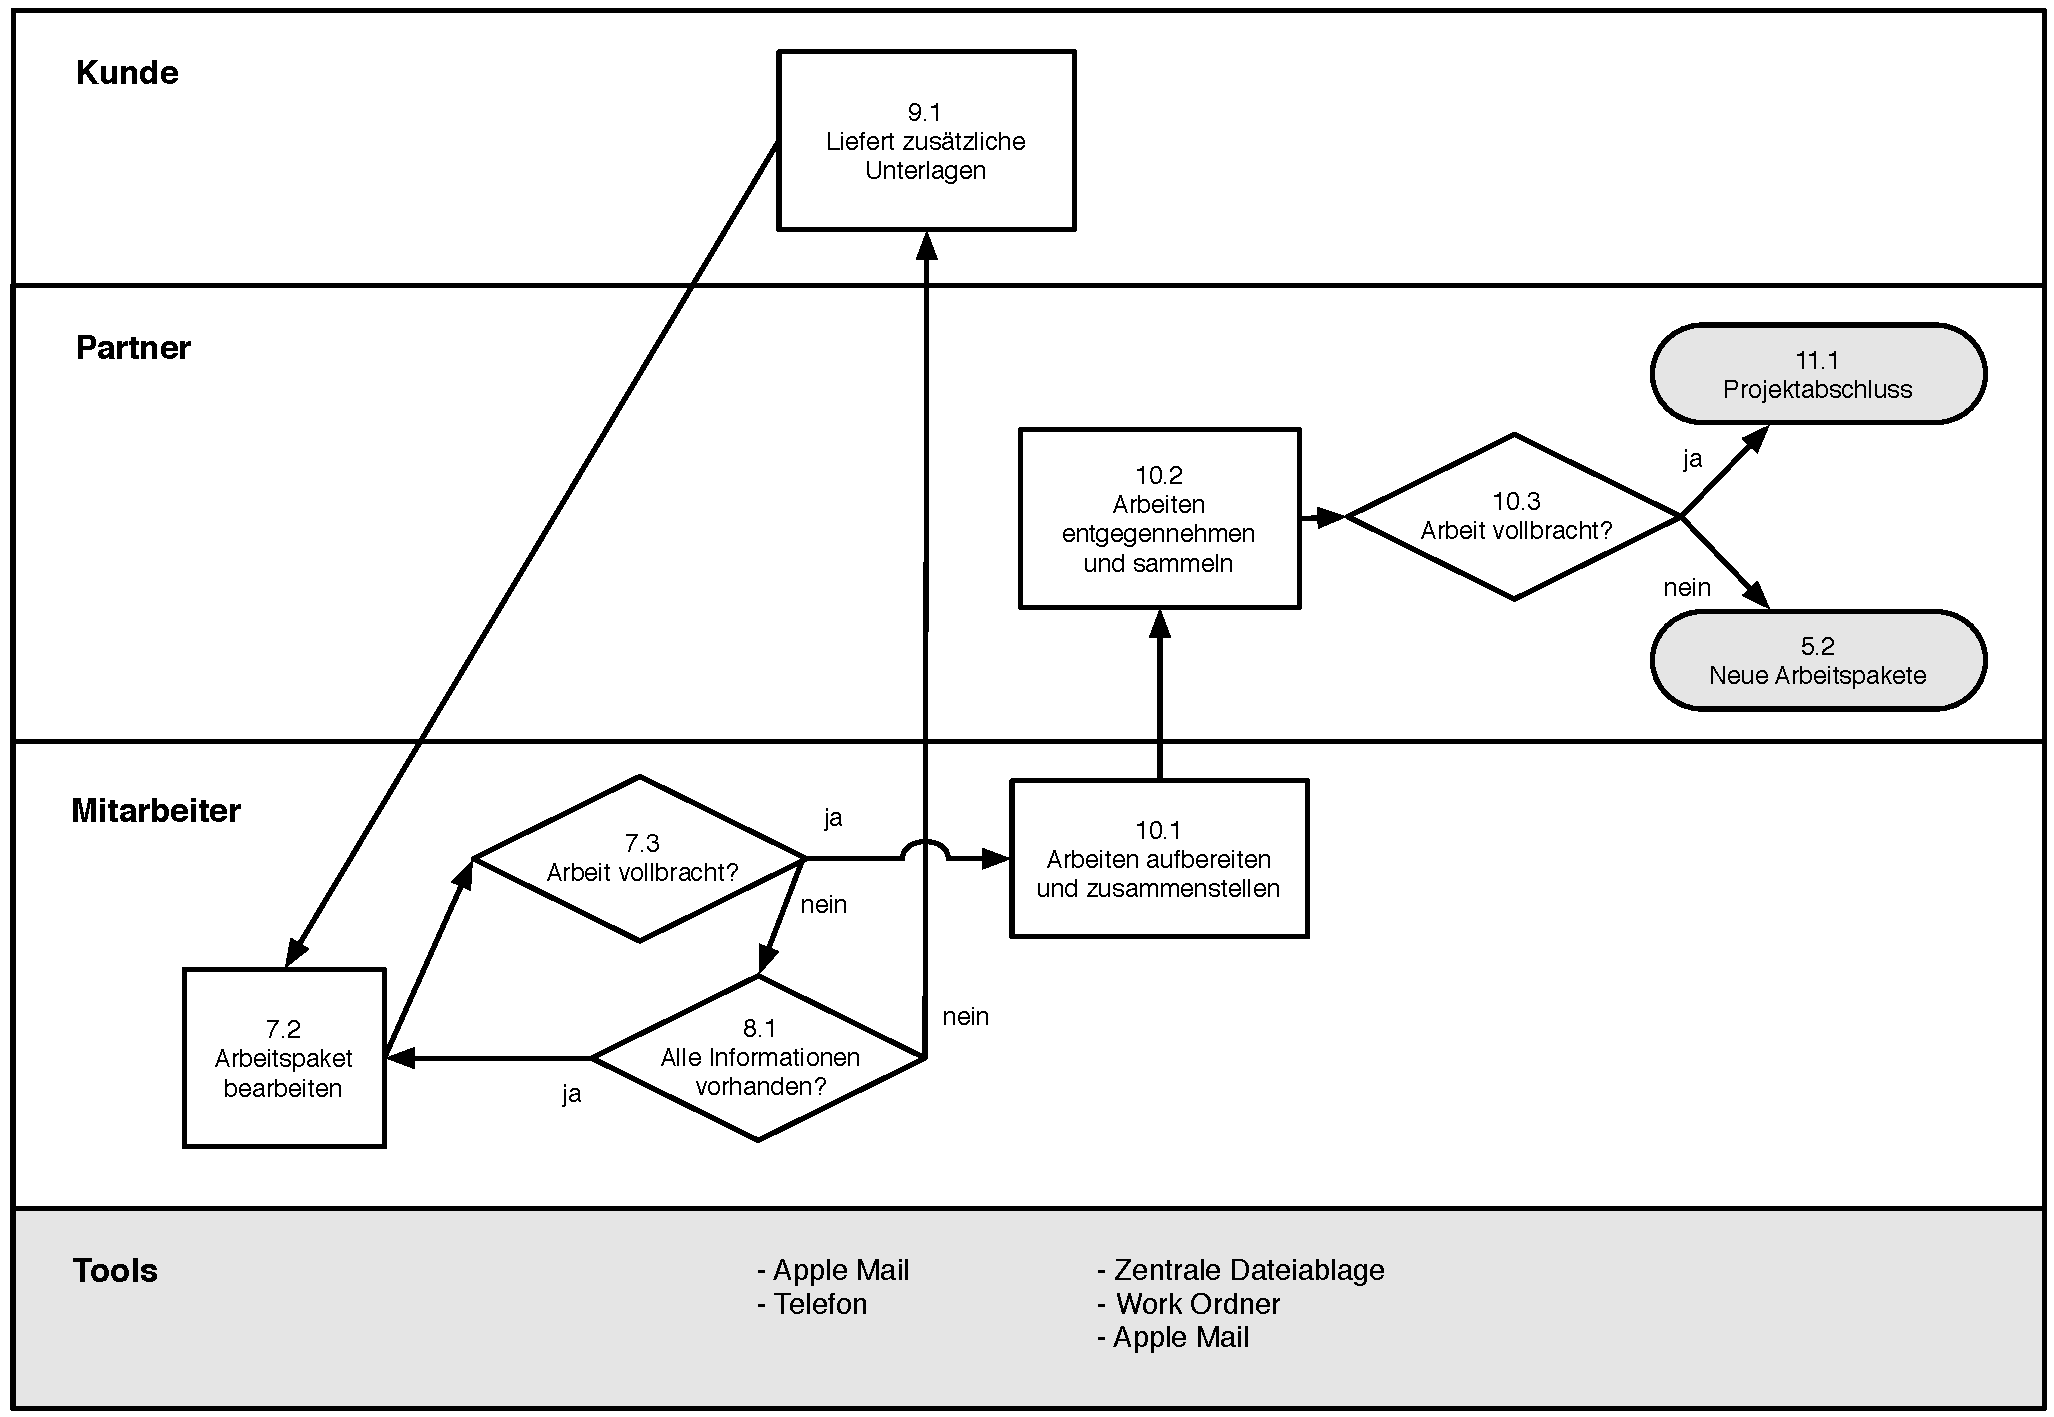
\includegraphics[width=0.99\textwidth,angle=0]{./bilder/analyse/02_ist_prozesse_arbeit_02.pdf}
\caption[Projektumsetzungs Prozess von allink 2/2]{Projektumsetzungs 
    Prozess von allink 2/2\footnotemark}
\label{pic:02_ist_prozesse_arbeit_02}
\end{center}
\end{figure}
\footnotetext{Eigene Darstellung}

In der ersten Phase der Projektdurchführung sammelt der Projektleiter bzw.
Partner alle nötigen Informationen, die zur Bearbeitung des Projektes notwendig sind.
Danach stellt er Arbeitspakete zusammen, die er wiederum an die Mitarbeiter verteilt.
Die Projektdurchführung ist in den Grafiken \ref{pic:02_ist_prozesse_arbeit_01} und 
\ref{pic:02_ist_prozesse_arbeit_02} grafisch dargestellt.

Der Partner verschafft sich einen überblick über das Projekt und gruppiert
die zu erledigenden Arbeiten in Arbeitspakete (\textbf{5.2}). Er besorgt alle nötigen Informationen
und Unterlagen, die zur Bewältigung eines Arbeitspaketes notwendig sind und fordert
bei Kunden wenn nötig noch mehr Informationen und Unterlagen ein (\textbf{6.1}).
Sind alle Informationen vorhanden (\textbf{5.3}) übergibt er die Arbeitspakete
den Mitarbeitern zur Erledigung.

Der Mitarbeiter nimmt das Arbeitspaket entgegen (\textbf{7.1}) und beginnt
mit dessen Bearbeitung (\textbf{7.2}). Stellt sich heraus, dass er sein Arbeitspaket
noch nicht abschliessen kann (\textbf{7.3}) und noch mehr Informationen oder
Unterlagen benötigt (\textbf{8.1}), kommt es oft vor, dass der Mitarbeiter
eigenständig beim Kunden zusätzliche Unterlagen einfordert (\textbf{9.1}).
Sobald er ein Paket abschliessen kann, stellt er alles Erarbeitete zusammen (\textbf{10.1})
und übergibt es dem zuständigen Partner bzw. Projektleiter.
Dieser nimmt alle Arbeitspakete entgegen (\textbf{10.2})
und überprüft diese (\textbf{10.3}). Sofern zusätzliche Arbeiten nötig sind,
stellt er diese wieder zusammen und der Bearbeitungsprozess beginnt von neuem (\textbf{5.2}).

Sind alle Arbeiten vollbracht, geht es über in den Projektabschluss (\textbf{11.1}). Dies wirkt
zu früh, da der Kunde bis zu diesem Zeitpunkt noch keine Ergebnisse gesehen
hat. In der Theorie ist die Produktabnahme jedoch auch im Projektabschluss angesiedelt.
Die Präsentation der Resultate und das Feedback des Kunden kommen darin zur Geltung. 
Geht man vom Optimalfall aus, kann das Projekt zu diesem Zeitpunk abgeschlossen 
werden. In der Praxis ist das vor allem bei kleineren Projekten der Fall, wie 
der Erstellung eines neuen Flyers\footnote{Mit einem Flyer bezeichnet man Flugblätter
die zum Transport von Werbebotschaften verwendet werden.}, bei dem sich das Konzept 
über Monate nicht geändert hat und nur Textkorrekturen und leichte visuelle 
Anpassungen notwendig sind. In den meisten Fällen aber kann mit Feedback des
Kunden gerechnet werden, das zu neuen Arbeitspaketen führt.

\clearpage

\subsection{Projektabschluss}

\begin{figure}[p]
\begin{center}
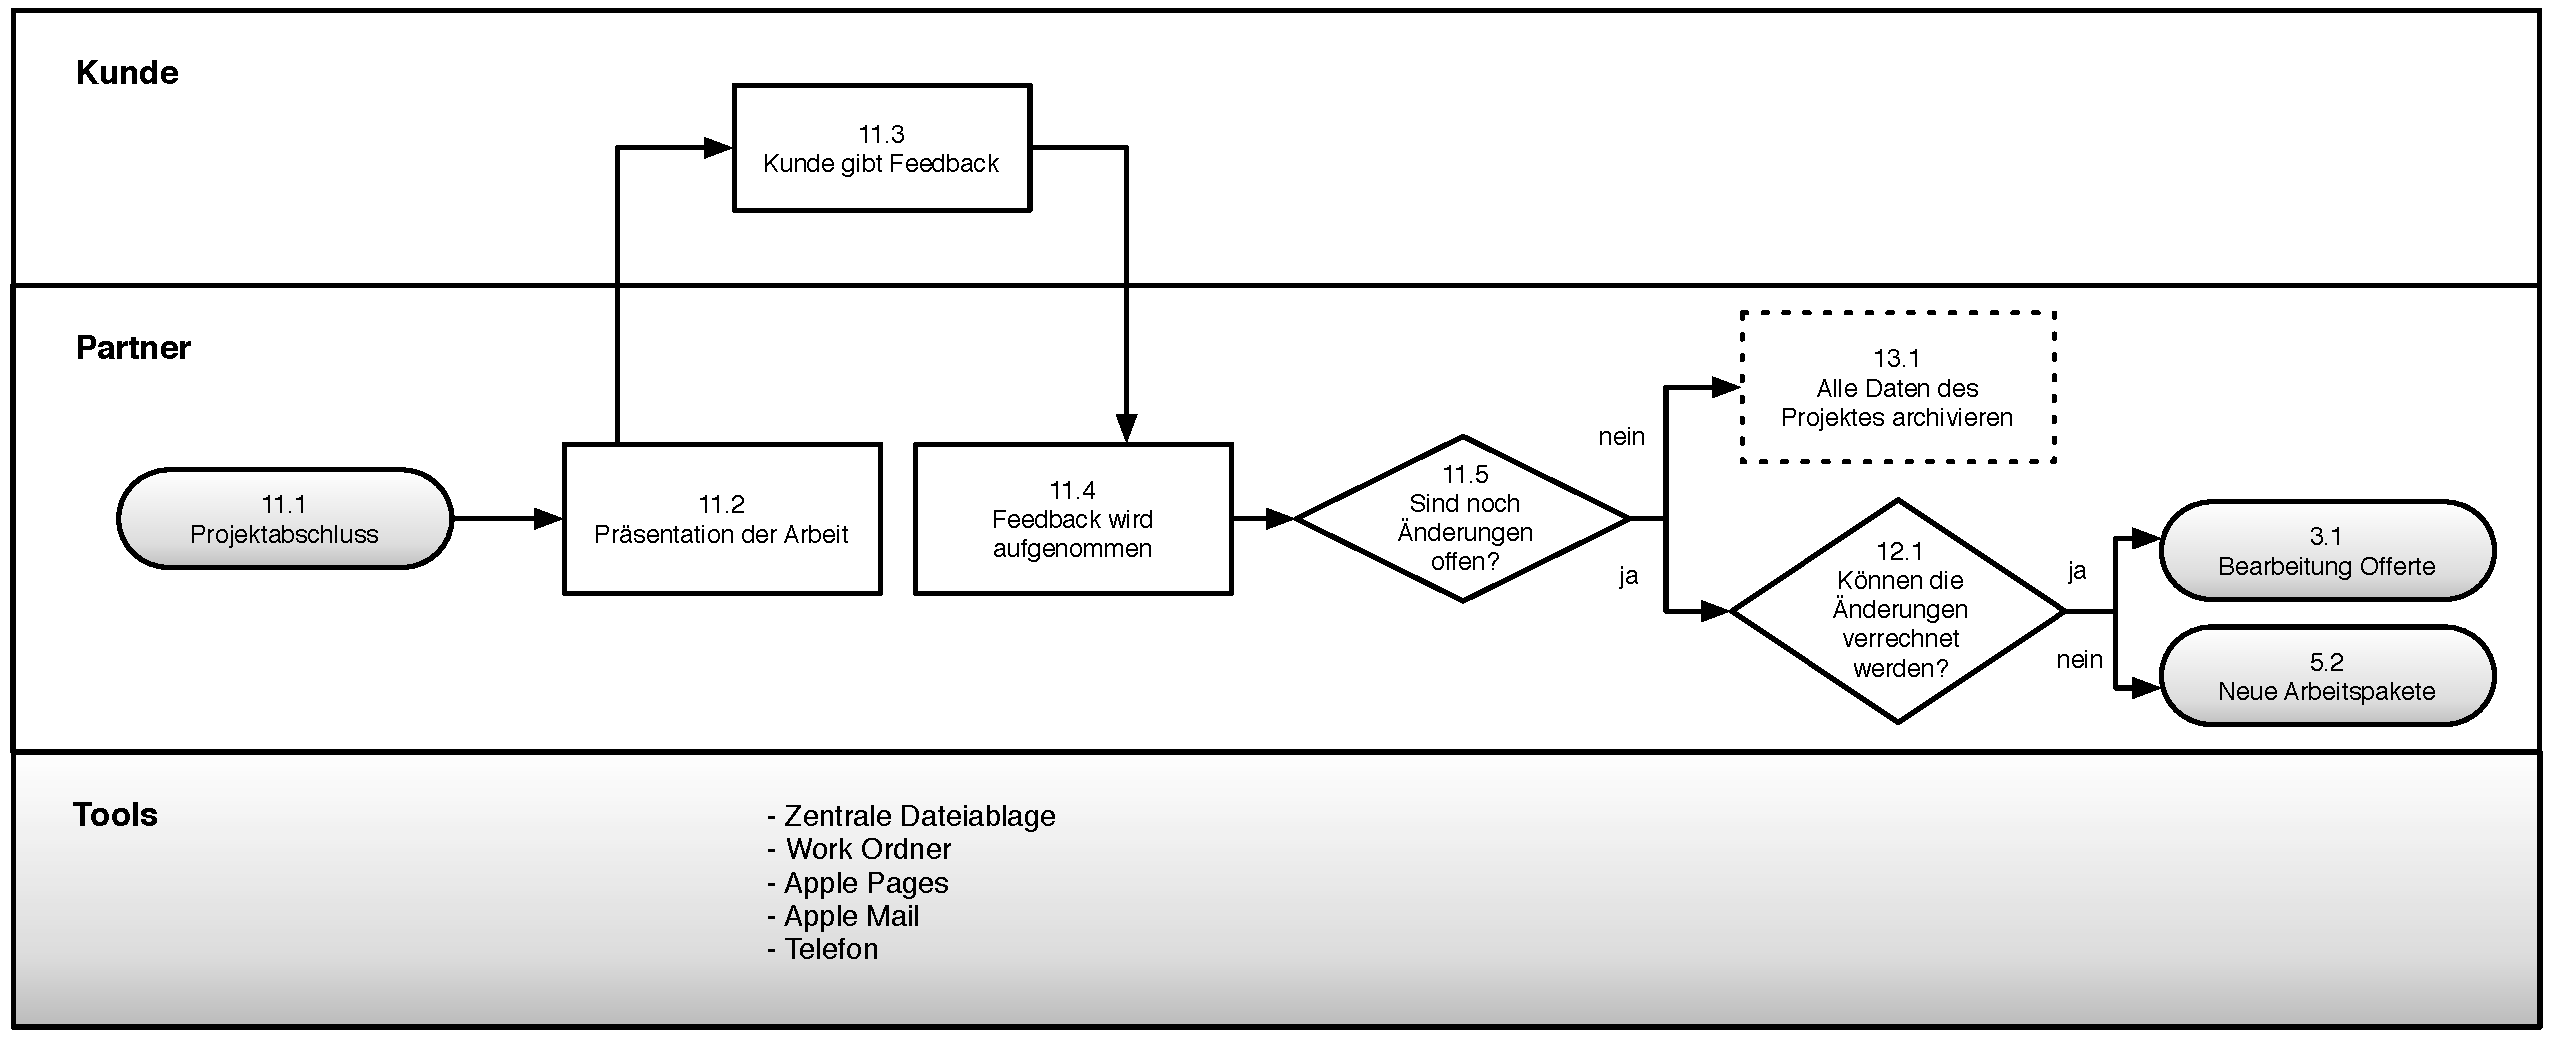
\includegraphics[width=0.99\textwidth,angle=0]{./bilder/analyse/03_ist_prozesse_abschluss_01.pdf}
\caption[Projektabschluss Prozess von allink 1/2]{Projektabschluss 
    Prozess von allink 1/2\footnotemark}
\label{pic:03_ist_prozesse_abschluss_01}
\end{center}
\end{figure}
\footnotetext{Eigene Darstellung}

\begin{figure}[p]
\begin{center}
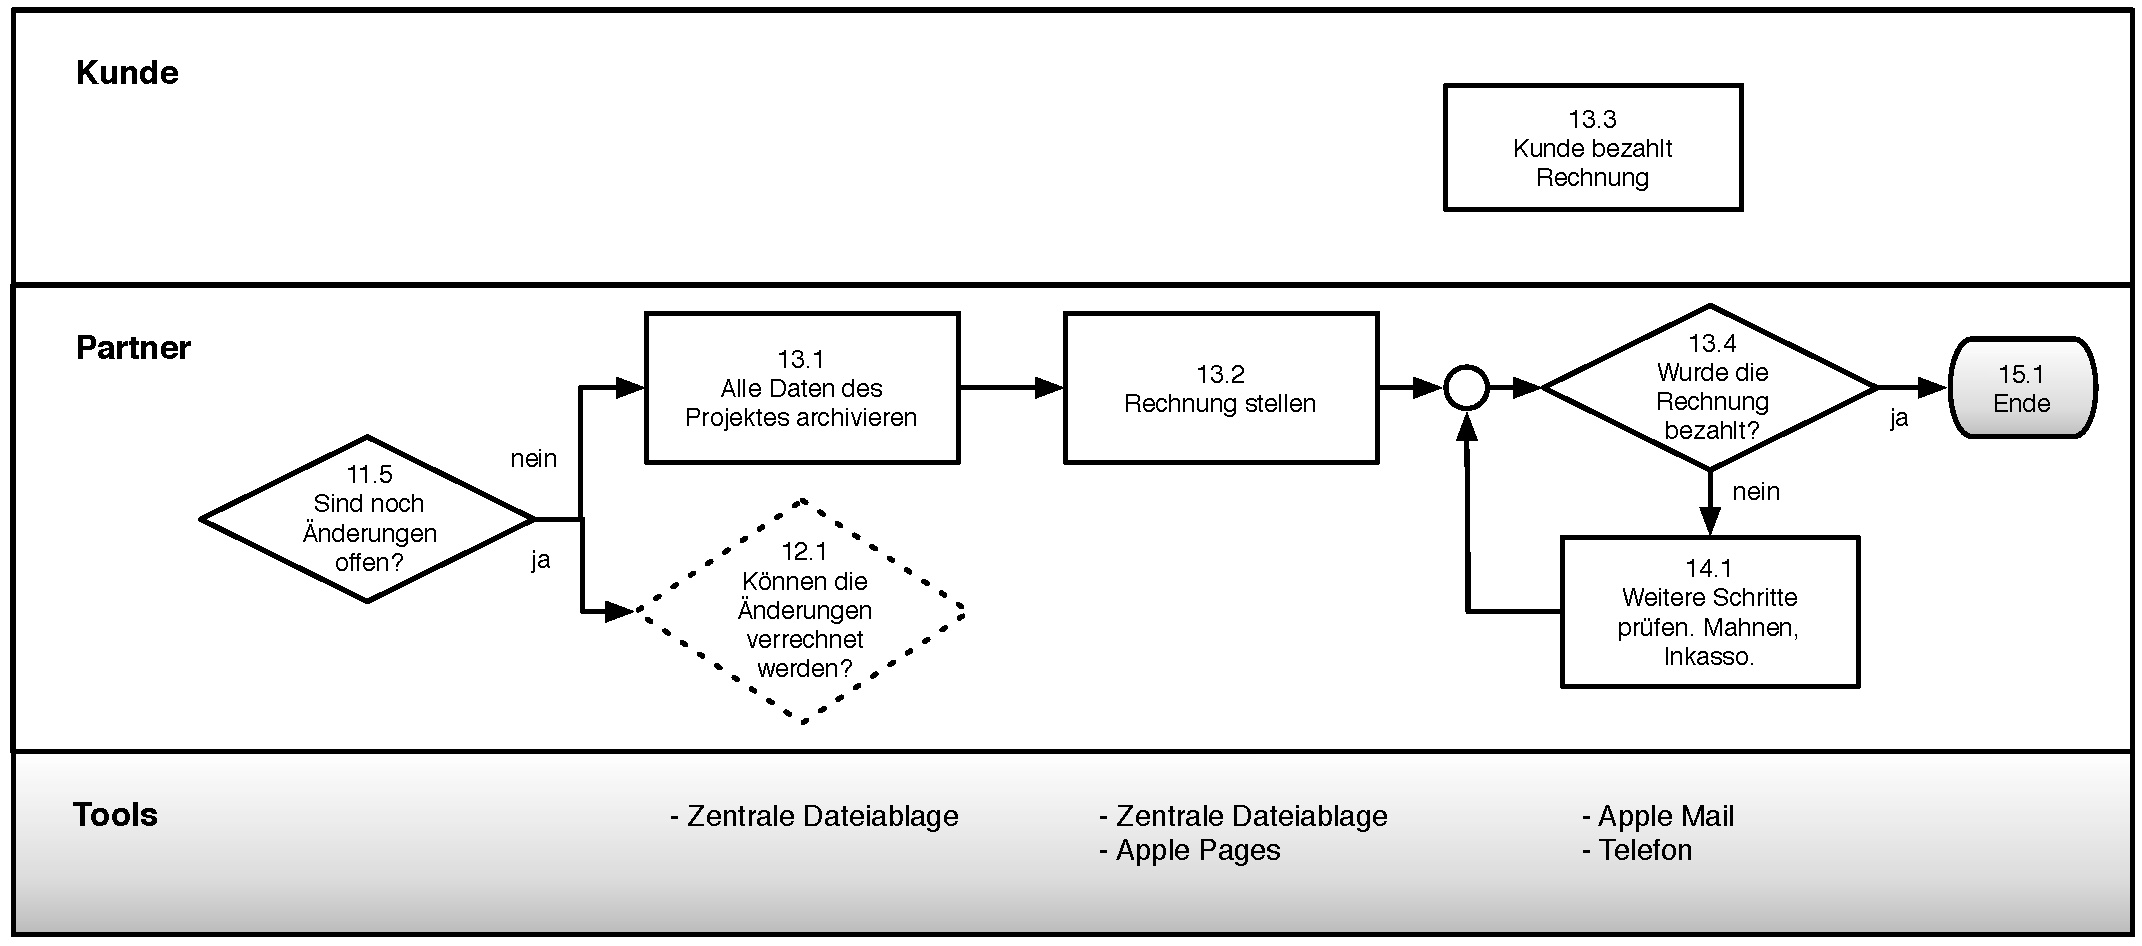
\includegraphics[width=0.99\textwidth,angle=0]{./bilder/analyse/03_ist_prozesse_abschluss_02.pdf}
\caption[Projektabschluss Prozess von allink 2/2]{Projektabschluss 
    Prozess von allink 2/2\footnotemark}
\label{pic:03_ist_prozesse_abschluss_02}
\end{center}
\end{figure}
\footnotetext{Eigene Darstellung}

In den Darstellungen \ref{pic:03_ist_prozesse_abschluss_01} und
\ref{pic:03_ist_prozesse_abschluss_02} ist der aktuelle Prozess des Projektabschlusses 
ersichtlich. Als erstes folgt nun die Präsentation der Arbeit beim Auftraggeber 
bzw. Kunden (\textbf{11.2}). Der Kunde gibt daraufhin Feedback (\textbf{11.3}), 
welches vom Projektleiter entgegengenommen und mit dem Kunden diskutiert wird (\textbf{11.4}).
Die in der Theorie empfohlenen Dokumente wie das Übergabe- und Übernahmeprotokoll
der Produktabnahme kommen zur Zeit gar nicht zur Anwendung.

Sofern dann noch Änderungen und Anpassungen nötig sind (\textbf{11.5}), stellt
der Projektleiter bzw. Partner wieder neuen Arbeitspakete zusammen und der
Bearbeitungsprozess beginnt von neuem (\textbf{5.2}). Wenn es sich bei den Wünschen
des Auftraggebers um neue, noch nicht bekannte, Anforderungen handelt, überprüft
der Partner ob eine Anpassung der Offerte nötig ist (\textbf{12.1}).

Hier liegt es im Ermessen des Partners, ob es sinnvoll ist die zusätzlichen Kosten 
selbst zu tragen oder in Rechnung zu stellen. Je nach Projektverlauf, auf Grund von
Verzögerungen oder sonstigen Unannehmlichkeiten für den Auftraggeber, kann es
von Nutzen sein dem Kunden zu diesem Zeitpunkt entgegen zu kommen.

Wenn der Auftraggeber zufrieden ist und keine weiteren Anpassungen nötig sind, 
werden alle Daten des Projektes archiviert (\textbf{13.1}). Danach wird die
Endabrechnung durchgeführt und die Abschlussrechnung in Rechnung gestellt (\textbf{13.2}).
Im Verlauf der Zahlungsfrist bezahlt der Kunde die Rechnung (\textbf{13.3}).
Dies wird so lange überwacht (\textbf{13.4}) bis alle offenen Rechnungen beglichen
sind. Wenn eine Rechnung nach der Zahlungsfrist nicht bezahlt wurde, wird
geprüft ob weitere Schritte nötig sind (\textbf{14.1}).

In den meisten Fällen reichen ein paar zusätzliche Tage oder das Nachfragen beim 
Kunden. In den wenigsten Fällen muss gemahnt werden und das Einschalten eines 
Inkassounternehmens war in der Geschichte von allink zum Glück erst ein einziges 
mal notwendig. Sobald alle Rechnungen beglichen sind, gilt das Projekt definitiv 
abgeschlossen (\textbf{15.1}).

Zu diesem Zeitpunkt geschieht das Sammeln der Erfahrungsdaten aus dem Projekt,
wie in der Theorie beschrieben, nur implizit. Die Daten werden also nicht in 
einer Erfahrungsdatenbank gespeichert sondern existieren nur in den Köpfen
der Projektmitarbeiter.

\clearpage
